\documentclass[twoside]{book}

% Packages required by doxygen
\usepackage{calc}
\usepackage{doxygen}
\usepackage{graphicx}
\usepackage[utf8]{inputenc}
\usepackage{makeidx}
\usepackage{multicol}
\usepackage{multirow}
\usepackage{textcomp}
\usepackage[table]{xcolor}

% Font selection
\usepackage[T1]{fontenc}
\usepackage{mathptmx}
\usepackage[scaled=.90]{helvet}
\usepackage{courier}
\usepackage{amssymb}
\usepackage{sectsty}
\renewcommand{\familydefault}{\sfdefault}
\allsectionsfont{%
  \fontseries{bc}\selectfont%
  \color{darkgray}%
}
\renewcommand{\DoxyLabelFont}{%
  \fontseries{bc}\selectfont%
  \color{darkgray}%
}

% Page & text layout
\usepackage{geometry}
\geometry{%
  a4paper,%
  top=2.5cm,%
  bottom=2.5cm,%
  left=2.5cm,%
  right=2.5cm%
}
\tolerance=750
\hfuzz=15pt
\hbadness=750
\setlength{\emergencystretch}{15pt}
\setlength{\parindent}{0cm}
\setlength{\parskip}{0.2cm}
\makeatletter
\renewcommand{\paragraph}{%
  \@startsection{paragraph}{4}{0ex}{-1.0ex}{1.0ex}{%
    \normalfont\normalsize\bfseries\SS@parafont%
  }%
}
\renewcommand{\subparagraph}{%
  \@startsection{subparagraph}{5}{0ex}{-1.0ex}{1.0ex}{%
    \normalfont\normalsize\bfseries\SS@subparafont%
  }%
}
\makeatother

% Headers & footers
\usepackage{fancyhdr}
\pagestyle{fancyplain}
\fancyhead[LE]{\fancyplain{}{\bfseries\thepage}}
\fancyhead[CE]{\fancyplain{}{}}
\fancyhead[RE]{\fancyplain{}{\bfseries\leftmark}}
\fancyhead[LO]{\fancyplain{}{\bfseries\rightmark}}
\fancyhead[CO]{\fancyplain{}{}}
\fancyhead[RO]{\fancyplain{}{\bfseries\thepage}}
\fancyfoot[LE]{\fancyplain{}{}}
\fancyfoot[CE]{\fancyplain{}{}}
\fancyfoot[RE]{\fancyplain{}{\bfseries\scriptsize Generated on Tue May 21 2013 15:13:13 for RoboControllerSDK by Doxygen }}
\fancyfoot[LO]{\fancyplain{}{\bfseries\scriptsize Generated on Tue May 21 2013 15:13:13 for RoboControllerSDK by Doxygen }}
\fancyfoot[CO]{\fancyplain{}{}}
\fancyfoot[RO]{\fancyplain{}{}}
\renewcommand{\footrulewidth}{0.4pt}
\renewcommand{\chaptermark}[1]{%
  \markboth{#1}{}%
}
\renewcommand{\sectionmark}[1]{%
  \markright{\thesection\ #1}%
}

% Indices & bibliography
\usepackage{natbib}
\usepackage[titles]{tocloft}
\setcounter{tocdepth}{3}
\setcounter{secnumdepth}{5}
\makeindex

% Hyperlinks (required, but should be loaded last)
\usepackage{ifpdf}
\ifpdf
  \usepackage[pdftex,pagebackref=true]{hyperref}
\else
  \usepackage[ps2pdf,pagebackref=true]{hyperref}
\fi
\hypersetup{%
  colorlinks=true,%
  linkcolor=blue,%
  citecolor=blue,%
  unicode%
}

% Custom commands
\newcommand{\clearemptydoublepage}{%
  \newpage{\pagestyle{empty}\cleardoublepage}%
}


%===== C O N T E N T S =====

\begin{document}

% Titlepage & ToC
\hypersetup{pageanchor=false}
\pagenumbering{roman}
\begin{titlepage}
\vspace*{7cm}
\begin{center}%
{\Large Robo\-Controller\-S\-D\-K }\\
\vspace*{1cm}
{\large Generated by Doxygen 1.8.4}\\
\vspace*{0.5cm}
{\small Tue May 21 2013 15:13:13}\\
\end{center}
\end{titlepage}
\clearemptydoublepage
\tableofcontents
\clearemptydoublepage
\pagenumbering{arabic}
\hypersetup{pageanchor=true}

%--- Begin generated contents ---
\chapter{Hierarchical Index}
\section{Class Hierarchy}
This inheritance list is sorted roughly, but not completely, alphabetically\-:\begin{DoxyCompactList}
\item \contentsline{section}{\-\_\-\-Board\-Status}{\pageref{struct___board_status}}{}
\item \contentsline{section}{\-\_\-\-Robot\-Configuration}{\pageref{struct___robot_configuration}}{}
\item Q\-Thread\begin{DoxyCompactList}
\item \contentsline{section}{roboctrl\-:\-:Robo\-Controller\-S\-D\-K}{\pageref{classroboctrl_1_1_robo_controller_s_d_k}}{}
\end{DoxyCompactList}
\item \contentsline{section}{roboctrl\-:\-:Rc\-Exception}{\pageref{classroboctrl_1_1_rc_exception}}{}
\end{DoxyCompactList}

\chapter{Class Index}
\section{Class List}
Here are the classes, structs, unions and interfaces with brief descriptions\-:\begin{DoxyCompactList}
\item\contentsline{section}{\hyperlink{struct___board_status}{\-\_\-\-Board\-Status} \\*Used to mantain the state of the configuration of the board }{\pageref{struct___board_status}}{}
\item\contentsline{section}{\hyperlink{struct___robot_configuration}{\-\_\-\-Robot\-Configuration} \\*Used to mantain the state of the configuration of the robot }{\pageref{struct___robot_configuration}}{}
\item\contentsline{section}{\hyperlink{classroboctrl_1_1_rc_exception}{roboctrl\-::\-Rc\-Exception} \\*A generic error exception that can be thrown by the application }{\pageref{classroboctrl_1_1_rc_exception}}{}
\item\contentsline{section}{\hyperlink{classroboctrl_1_1_robo_controller_s_d_k}{roboctrl\-::\-Robo\-Controller\-S\-D\-K} }{\pageref{classroboctrl_1_1_robo_controller_s_d_k}}{}
\end{DoxyCompactList}

\chapter{Class Documentation}
\hypertarget{struct___board_status}{\section{\-\_\-\-Board\-Status Struct Reference}
\label{struct___board_status}\index{\-\_\-\-Board\-Status@{\-\_\-\-Board\-Status}}
}


Used to mantain the state of the configuration of the board.  




{\ttfamily \#include $<$Robo\-Controller\-S\-D\-K\-\_\-global.\-h$>$}

\subsection*{Public Attributes}
\begin{DoxyCompactItemize}
\item 
bool \hyperlink{struct___board_status_ab46b9c91875df3c2871962e1b5d7ac59}{pid\-Enable}
\item 
bool \hyperlink{struct___board_status_aacf5e62d8821a7ee164979f9f529a867}{wd\-Enable}
\item 
bool \hyperlink{struct___board_status_a30b34c999564107e05997c953d0fc31c}{save\-To\-Eeprom}
\item 
bool \hyperlink{struct___board_status_a950c73606e91c9302fde6d119f7e79a8}{accel\-Ramp\-Enable}
\end{DoxyCompactItemize}


\subsection{Detailed Description}
Used to mantain the state of the configuration of the board. 

\subsection{Member Data Documentation}
\hypertarget{struct___board_status_a950c73606e91c9302fde6d119f7e79a8}{\index{\-\_\-\-Board\-Status@{\-\_\-\-Board\-Status}!accel\-Ramp\-Enable@{accel\-Ramp\-Enable}}
\index{accel\-Ramp\-Enable@{accel\-Ramp\-Enable}!_BoardStatus@{\-\_\-\-Board\-Status}}
\subsubsection[{accel\-Ramp\-Enable}]{\setlength{\rightskip}{0pt plus 5cm}bool \-\_\-\-Board\-Status\-::accel\-Ramp\-Enable}}\label{struct___board_status_a950c73606e91c9302fde6d119f7e79a8}
Indicates if acceleration is limited by speed ramps \hypertarget{struct___board_status_ab46b9c91875df3c2871962e1b5d7ac59}{\index{\-\_\-\-Board\-Status@{\-\_\-\-Board\-Status}!pid\-Enable@{pid\-Enable}}
\index{pid\-Enable@{pid\-Enable}!_BoardStatus@{\-\_\-\-Board\-Status}}
\subsubsection[{pid\-Enable}]{\setlength{\rightskip}{0pt plus 5cm}bool \-\_\-\-Board\-Status\-::pid\-Enable}}\label{struct___board_status_ab46b9c91875df3c2871962e1b5d7ac59}
Indicates if the motor P\-I\-D controls are enabled \hypertarget{struct___board_status_a30b34c999564107e05997c953d0fc31c}{\index{\-\_\-\-Board\-Status@{\-\_\-\-Board\-Status}!save\-To\-Eeprom@{save\-To\-Eeprom}}
\index{save\-To\-Eeprom@{save\-To\-Eeprom}!_BoardStatus@{\-\_\-\-Board\-Status}}
\subsubsection[{save\-To\-Eeprom}]{\setlength{\rightskip}{0pt plus 5cm}bool \-\_\-\-Board\-Status\-::save\-To\-Eeprom}}\label{struct___board_status_a30b34c999564107e05997c953d0fc31c}
Indicates if the Board parameters are saved to Eeprom when changed \hypertarget{struct___board_status_aacf5e62d8821a7ee164979f9f529a867}{\index{\-\_\-\-Board\-Status@{\-\_\-\-Board\-Status}!wd\-Enable@{wd\-Enable}}
\index{wd\-Enable@{wd\-Enable}!_BoardStatus@{\-\_\-\-Board\-Status}}
\subsubsection[{wd\-Enable}]{\setlength{\rightskip}{0pt plus 5cm}bool \-\_\-\-Board\-Status\-::wd\-Enable}}\label{struct___board_status_aacf5e62d8821a7ee164979f9f529a867}
Indicates if the Command Watch\-Dod is enabled. If it is true and the board does not receive command for N msec (get\-Watch\-Dog\-Time and set\-Watch\-Dog\-Time)the motors stop 

The documentation for this struct was generated from the following file\-:\begin{DoxyCompactItemize}
\item 
Robo\-Controller\-S\-D\-K\-\_\-global.\-h\end{DoxyCompactItemize}

\hypertarget{struct___robot_configuration}{\section{\-\_\-\-Robot\-Configuration Struct Reference}
\label{struct___robot_configuration}\index{\-\_\-\-Robot\-Configuration@{\-\_\-\-Robot\-Configuration}}
}


Used to mantain the state of the configuration of the robot.  




{\ttfamily \#include $<$Robo\-Controller\-S\-D\-K\-\_\-global.\-h$>$}

\subsection*{Public Attributes}
\begin{DoxyCompactItemize}
\item 
quint16 \hyperlink{struct___robot_configuration_a9aa2a32a66e3d9559e9b43ccef43e74b}{Weight}
\item 
quint16 \hyperlink{struct___robot_configuration_ab9fcfe56d6fe56d0e7738e51dbcd062b}{Width}
\item 
quint16 \hyperlink{struct___robot_configuration_afb09adbb9fd458bb18c9aa2dd25b9be0}{Height}
\item 
quint16 \hyperlink{struct___robot_configuration_ab61562623c27b882ecb55262336efb96}{Lenght}
\item 
quint16 \hyperlink{struct___robot_configuration_ad18b7c6607d189b0507c67f584d7213c}{Wheel\-Base}
\item 
quint16 \hyperlink{struct___robot_configuration_a4fba24bbead4c38e30182570a9fc111b}{Wheel\-Radius\-Left}
\item 
quint16 \hyperlink{struct___robot_configuration_a0cd7d7ca4eea7abb6c751f16a268a22c}{Wheel\-Radius\-Right}
\item 
quint16 \hyperlink{struct___robot_configuration_af182347d3c875e986ba720760ef55a54}{Encoder\-Cpr\-Left}
\item 
quint16 \hyperlink{struct___robot_configuration_a63e2c47bb9763838aa3b1b097890a5a5}{Encoder\-Cpr\-Right}
\item 
quint16 \hyperlink{struct___robot_configuration_a2a12b5f279876cf7dac9ab2d1129d793}{Max\-Rpm\-Motor\-Left}
\item 
quint16 \hyperlink{struct___robot_configuration_a410e871a1f0c5d0a9a06f57f584b1407}{Max\-Rpm\-Motor\-Right}
\item 
quint16 \hyperlink{struct___robot_configuration_ab7e58c3cd60604b5965a432eb3e483a4}{Max\-Ampere\-Motor\-Left}
\item 
quint16 \hyperlink{struct___robot_configuration_a42620d2d390b5647ad91080099804f24}{Max\-Ampere\-Motor\-Right}
\item 
quint16 \hyperlink{struct___robot_configuration_a5c556f8da91c14e17b2150f5b9a9ed26}{Max\-Torque\-Motor\-Left}
\item 
quint16 \hyperlink{struct___robot_configuration_a3d3d5e740395408ba0ee9d108c68fcb9}{Max\-Torque\-Motor\-Right}
\item 
quint16 \hyperlink{struct___robot_configuration_a79de71ac2a7be019acea88d1cb1c92cc}{Ratio\-Shaft\-Left}
\item 
quint16 \hyperlink{struct___robot_configuration_aef75f196a9ac7433f73b13c8be32ee50}{Ratio\-Shaft\-Right}
\item 
quint16 \hyperlink{struct___robot_configuration_a6e49cb2f07852f96c80c4466a20b4334}{Ratio\-Motor\-Left}
\item 
quint16 \hyperlink{struct___robot_configuration_ac89f6df8e7eb18f6535a2f46c6ff2895}{Ratio\-Motor\-Right}
\item 
Pin\-Level \hyperlink{struct___robot_configuration_a44c8ef3ff07fc7f7c00489b76c73e738}{Motor\-Enable\-Level}
\item 
Encoder\-Pos \hyperlink{struct___robot_configuration_a5a5010ca51d595bec652a274216e8d8e}{Encoder\-Position}
\end{DoxyCompactItemize}


\subsection{Detailed Description}
Used to mantain the state of the configuration of the robot. 

\subsection{Member Data Documentation}
\hypertarget{struct___robot_configuration_af182347d3c875e986ba720760ef55a54}{\index{\-\_\-\-Robot\-Configuration@{\-\_\-\-Robot\-Configuration}!Encoder\-Cpr\-Left@{Encoder\-Cpr\-Left}}
\index{Encoder\-Cpr\-Left@{Encoder\-Cpr\-Left}!_RobotConfiguration@{\-\_\-\-Robot\-Configuration}}
\subsubsection[{Encoder\-Cpr\-Left}]{\setlength{\rightskip}{0pt plus 5cm}quint16 \-\_\-\-Robot\-Configuration\-::\-Encoder\-Cpr\-Left}}\label{struct___robot_configuration_af182347d3c875e986ba720760ef55a54}
Count per Round of the left encoder \hypertarget{struct___robot_configuration_a63e2c47bb9763838aa3b1b097890a5a5}{\index{\-\_\-\-Robot\-Configuration@{\-\_\-\-Robot\-Configuration}!Encoder\-Cpr\-Right@{Encoder\-Cpr\-Right}}
\index{Encoder\-Cpr\-Right@{Encoder\-Cpr\-Right}!_RobotConfiguration@{\-\_\-\-Robot\-Configuration}}
\subsubsection[{Encoder\-Cpr\-Right}]{\setlength{\rightskip}{0pt plus 5cm}quint16 \-\_\-\-Robot\-Configuration\-::\-Encoder\-Cpr\-Right}}\label{struct___robot_configuration_a63e2c47bb9763838aa3b1b097890a5a5}
Count per Round of the right encoder \hypertarget{struct___robot_configuration_a5a5010ca51d595bec652a274216e8d8e}{\index{\-\_\-\-Robot\-Configuration@{\-\_\-\-Robot\-Configuration}!Encoder\-Position@{Encoder\-Position}}
\index{Encoder\-Position@{Encoder\-Position}!_RobotConfiguration@{\-\_\-\-Robot\-Configuration}}
\subsubsection[{Encoder\-Position}]{\setlength{\rightskip}{0pt plus 5cm}Encoder\-Pos \-\_\-\-Robot\-Configuration\-::\-Encoder\-Position}}\label{struct___robot_configuration_a5a5010ca51d595bec652a274216e8d8e}
Encoder on the shaft of the motor or of the wheel \hypertarget{struct___robot_configuration_afb09adbb9fd458bb18c9aa2dd25b9be0}{\index{\-\_\-\-Robot\-Configuration@{\-\_\-\-Robot\-Configuration}!Height@{Height}}
\index{Height@{Height}!_RobotConfiguration@{\-\_\-\-Robot\-Configuration}}
\subsubsection[{Height}]{\setlength{\rightskip}{0pt plus 5cm}quint16 \-\_\-\-Robot\-Configuration\-::\-Height}}\label{struct___robot_configuration_afb09adbb9fd458bb18c9aa2dd25b9be0}
Robot Height (mm) \hypertarget{struct___robot_configuration_ab61562623c27b882ecb55262336efb96}{\index{\-\_\-\-Robot\-Configuration@{\-\_\-\-Robot\-Configuration}!Lenght@{Lenght}}
\index{Lenght@{Lenght}!_RobotConfiguration@{\-\_\-\-Robot\-Configuration}}
\subsubsection[{Lenght}]{\setlength{\rightskip}{0pt plus 5cm}quint16 \-\_\-\-Robot\-Configuration\-::\-Lenght}}\label{struct___robot_configuration_ab61562623c27b882ecb55262336efb96}
Robot Lenght (mm) \hypertarget{struct___robot_configuration_ab7e58c3cd60604b5965a432eb3e483a4}{\index{\-\_\-\-Robot\-Configuration@{\-\_\-\-Robot\-Configuration}!Max\-Ampere\-Motor\-Left@{Max\-Ampere\-Motor\-Left}}
\index{Max\-Ampere\-Motor\-Left@{Max\-Ampere\-Motor\-Left}!_RobotConfiguration@{\-\_\-\-Robot\-Configuration}}
\subsubsection[{Max\-Ampere\-Motor\-Left}]{\setlength{\rightskip}{0pt plus 5cm}quint16 \-\_\-\-Robot\-Configuration\-::\-Max\-Ampere\-Motor\-Left}}\label{struct___robot_configuration_ab7e58c3cd60604b5965a432eb3e483a4}
Max current assorbed by left motor (m\-A) \hypertarget{struct___robot_configuration_a42620d2d390b5647ad91080099804f24}{\index{\-\_\-\-Robot\-Configuration@{\-\_\-\-Robot\-Configuration}!Max\-Ampere\-Motor\-Right@{Max\-Ampere\-Motor\-Right}}
\index{Max\-Ampere\-Motor\-Right@{Max\-Ampere\-Motor\-Right}!_RobotConfiguration@{\-\_\-\-Robot\-Configuration}}
\subsubsection[{Max\-Ampere\-Motor\-Right}]{\setlength{\rightskip}{0pt plus 5cm}quint16 \-\_\-\-Robot\-Configuration\-::\-Max\-Ampere\-Motor\-Right}}\label{struct___robot_configuration_a42620d2d390b5647ad91080099804f24}
Max current assorbed by right motor (m\-A) \hypertarget{struct___robot_configuration_a2a12b5f279876cf7dac9ab2d1129d793}{\index{\-\_\-\-Robot\-Configuration@{\-\_\-\-Robot\-Configuration}!Max\-Rpm\-Motor\-Left@{Max\-Rpm\-Motor\-Left}}
\index{Max\-Rpm\-Motor\-Left@{Max\-Rpm\-Motor\-Left}!_RobotConfiguration@{\-\_\-\-Robot\-Configuration}}
\subsubsection[{Max\-Rpm\-Motor\-Left}]{\setlength{\rightskip}{0pt plus 5cm}quint16 \-\_\-\-Robot\-Configuration\-::\-Max\-Rpm\-Motor\-Left}}\label{struct___robot_configuration_a2a12b5f279876cf7dac9ab2d1129d793}
Max R\-P\-M of the left motor \hypertarget{struct___robot_configuration_a410e871a1f0c5d0a9a06f57f584b1407}{\index{\-\_\-\-Robot\-Configuration@{\-\_\-\-Robot\-Configuration}!Max\-Rpm\-Motor\-Right@{Max\-Rpm\-Motor\-Right}}
\index{Max\-Rpm\-Motor\-Right@{Max\-Rpm\-Motor\-Right}!_RobotConfiguration@{\-\_\-\-Robot\-Configuration}}
\subsubsection[{Max\-Rpm\-Motor\-Right}]{\setlength{\rightskip}{0pt plus 5cm}quint16 \-\_\-\-Robot\-Configuration\-::\-Max\-Rpm\-Motor\-Right}}\label{struct___robot_configuration_a410e871a1f0c5d0a9a06f57f584b1407}
Max R\-P\-M of the right motor \hypertarget{struct___robot_configuration_a5c556f8da91c14e17b2150f5b9a9ed26}{\index{\-\_\-\-Robot\-Configuration@{\-\_\-\-Robot\-Configuration}!Max\-Torque\-Motor\-Left@{Max\-Torque\-Motor\-Left}}
\index{Max\-Torque\-Motor\-Left@{Max\-Torque\-Motor\-Left}!_RobotConfiguration@{\-\_\-\-Robot\-Configuration}}
\subsubsection[{Max\-Torque\-Motor\-Left}]{\setlength{\rightskip}{0pt plus 5cm}quint16 \-\_\-\-Robot\-Configuration\-::\-Max\-Torque\-Motor\-Left}}\label{struct___robot_configuration_a5c556f8da91c14e17b2150f5b9a9ed26}
Max torque of the left motor (Ncm) \hypertarget{struct___robot_configuration_a3d3d5e740395408ba0ee9d108c68fcb9}{\index{\-\_\-\-Robot\-Configuration@{\-\_\-\-Robot\-Configuration}!Max\-Torque\-Motor\-Right@{Max\-Torque\-Motor\-Right}}
\index{Max\-Torque\-Motor\-Right@{Max\-Torque\-Motor\-Right}!_RobotConfiguration@{\-\_\-\-Robot\-Configuration}}
\subsubsection[{Max\-Torque\-Motor\-Right}]{\setlength{\rightskip}{0pt plus 5cm}quint16 \-\_\-\-Robot\-Configuration\-::\-Max\-Torque\-Motor\-Right}}\label{struct___robot_configuration_a3d3d5e740395408ba0ee9d108c68fcb9}
Max torque of the right motor (Ncm) \hypertarget{struct___robot_configuration_a44c8ef3ff07fc7f7c00489b76c73e738}{\index{\-\_\-\-Robot\-Configuration@{\-\_\-\-Robot\-Configuration}!Motor\-Enable\-Level@{Motor\-Enable\-Level}}
\index{Motor\-Enable\-Level@{Motor\-Enable\-Level}!_RobotConfiguration@{\-\_\-\-Robot\-Configuration}}
\subsubsection[{Motor\-Enable\-Level}]{\setlength{\rightskip}{0pt plus 5cm}Pin\-Level \-\_\-\-Robot\-Configuration\-::\-Motor\-Enable\-Level}}\label{struct___robot_configuration_a44c8ef3ff07fc7f7c00489b76c73e738}
Enable Level of the Robot Driver (Low/\-High) \hypertarget{struct___robot_configuration_a6e49cb2f07852f96c80c4466a20b4334}{\index{\-\_\-\-Robot\-Configuration@{\-\_\-\-Robot\-Configuration}!Ratio\-Motor\-Left@{Ratio\-Motor\-Left}}
\index{Ratio\-Motor\-Left@{Ratio\-Motor\-Left}!_RobotConfiguration@{\-\_\-\-Robot\-Configuration}}
\subsubsection[{Ratio\-Motor\-Left}]{\setlength{\rightskip}{0pt plus 5cm}quint16 \-\_\-\-Robot\-Configuration\-::\-Ratio\-Motor\-Left}}\label{struct___robot_configuration_a6e49cb2f07852f96c80c4466a20b4334}
Reduction Ratio on the left Motor Shaft (Put 1 if you set Max R\-P\-M considering it just reduced) \hypertarget{struct___robot_configuration_ac89f6df8e7eb18f6535a2f46c6ff2895}{\index{\-\_\-\-Robot\-Configuration@{\-\_\-\-Robot\-Configuration}!Ratio\-Motor\-Right@{Ratio\-Motor\-Right}}
\index{Ratio\-Motor\-Right@{Ratio\-Motor\-Right}!_RobotConfiguration@{\-\_\-\-Robot\-Configuration}}
\subsubsection[{Ratio\-Motor\-Right}]{\setlength{\rightskip}{0pt plus 5cm}quint16 \-\_\-\-Robot\-Configuration\-::\-Ratio\-Motor\-Right}}\label{struct___robot_configuration_ac89f6df8e7eb18f6535a2f46c6ff2895}
Reduction Ratio on the right Motor Shaft (Put 1 if you set Max R\-P\-M considering it just reduced) \hypertarget{struct___robot_configuration_a79de71ac2a7be019acea88d1cb1c92cc}{\index{\-\_\-\-Robot\-Configuration@{\-\_\-\-Robot\-Configuration}!Ratio\-Shaft\-Left@{Ratio\-Shaft\-Left}}
\index{Ratio\-Shaft\-Left@{Ratio\-Shaft\-Left}!_RobotConfiguration@{\-\_\-\-Robot\-Configuration}}
\subsubsection[{Ratio\-Shaft\-Left}]{\setlength{\rightskip}{0pt plus 5cm}quint16 \-\_\-\-Robot\-Configuration\-::\-Ratio\-Shaft\-Left}}\label{struct___robot_configuration_a79de71ac2a7be019acea88d1cb1c92cc}
Reduction Ratio from the shaft of the left motor to the shaft of the left wheel \hypertarget{struct___robot_configuration_aef75f196a9ac7433f73b13c8be32ee50}{\index{\-\_\-\-Robot\-Configuration@{\-\_\-\-Robot\-Configuration}!Ratio\-Shaft\-Right@{Ratio\-Shaft\-Right}}
\index{Ratio\-Shaft\-Right@{Ratio\-Shaft\-Right}!_RobotConfiguration@{\-\_\-\-Robot\-Configuration}}
\subsubsection[{Ratio\-Shaft\-Right}]{\setlength{\rightskip}{0pt plus 5cm}quint16 \-\_\-\-Robot\-Configuration\-::\-Ratio\-Shaft\-Right}}\label{struct___robot_configuration_aef75f196a9ac7433f73b13c8be32ee50}
Reduction Ratio from the shaft of the right motor to the shaft of the right wheel \hypertarget{struct___robot_configuration_a9aa2a32a66e3d9559e9b43ccef43e74b}{\index{\-\_\-\-Robot\-Configuration@{\-\_\-\-Robot\-Configuration}!Weight@{Weight}}
\index{Weight@{Weight}!_RobotConfiguration@{\-\_\-\-Robot\-Configuration}}
\subsubsection[{Weight}]{\setlength{\rightskip}{0pt plus 5cm}quint16 \-\_\-\-Robot\-Configuration\-::\-Weight}}\label{struct___robot_configuration_a9aa2a32a66e3d9559e9b43ccef43e74b}
Robot Weight (g) \hypertarget{struct___robot_configuration_ad18b7c6607d189b0507c67f584d7213c}{\index{\-\_\-\-Robot\-Configuration@{\-\_\-\-Robot\-Configuration}!Wheel\-Base@{Wheel\-Base}}
\index{Wheel\-Base@{Wheel\-Base}!_RobotConfiguration@{\-\_\-\-Robot\-Configuration}}
\subsubsection[{Wheel\-Base}]{\setlength{\rightskip}{0pt plus 5cm}quint16 \-\_\-\-Robot\-Configuration\-::\-Wheel\-Base}}\label{struct___robot_configuration_ad18b7c6607d189b0507c67f584d7213c}
Distance between the center of the Wheels (mm) \hypertarget{struct___robot_configuration_a4fba24bbead4c38e30182570a9fc111b}{\index{\-\_\-\-Robot\-Configuration@{\-\_\-\-Robot\-Configuration}!Wheel\-Radius\-Left@{Wheel\-Radius\-Left}}
\index{Wheel\-Radius\-Left@{Wheel\-Radius\-Left}!_RobotConfiguration@{\-\_\-\-Robot\-Configuration}}
\subsubsection[{Wheel\-Radius\-Left}]{\setlength{\rightskip}{0pt plus 5cm}quint16 \-\_\-\-Robot\-Configuration\-::\-Wheel\-Radius\-Left}}\label{struct___robot_configuration_a4fba24bbead4c38e30182570a9fc111b}
Radius of the left wheel (0.\-01mm) \hypertarget{struct___robot_configuration_a0cd7d7ca4eea7abb6c751f16a268a22c}{\index{\-\_\-\-Robot\-Configuration@{\-\_\-\-Robot\-Configuration}!Wheel\-Radius\-Right@{Wheel\-Radius\-Right}}
\index{Wheel\-Radius\-Right@{Wheel\-Radius\-Right}!_RobotConfiguration@{\-\_\-\-Robot\-Configuration}}
\subsubsection[{Wheel\-Radius\-Right}]{\setlength{\rightskip}{0pt plus 5cm}quint16 \-\_\-\-Robot\-Configuration\-::\-Wheel\-Radius\-Right}}\label{struct___robot_configuration_a0cd7d7ca4eea7abb6c751f16a268a22c}
Radius of the right wheel (0.\-01mm) \hypertarget{struct___robot_configuration_ab9fcfe56d6fe56d0e7738e51dbcd062b}{\index{\-\_\-\-Robot\-Configuration@{\-\_\-\-Robot\-Configuration}!Width@{Width}}
\index{Width@{Width}!_RobotConfiguration@{\-\_\-\-Robot\-Configuration}}
\subsubsection[{Width}]{\setlength{\rightskip}{0pt plus 5cm}quint16 \-\_\-\-Robot\-Configuration\-::\-Width}}\label{struct___robot_configuration_ab9fcfe56d6fe56d0e7738e51dbcd062b}
Robot Width (mm) 

The documentation for this struct was generated from the following file\-:\begin{DoxyCompactItemize}
\item 
Robo\-Controller\-S\-D\-K\-\_\-global.\-h\end{DoxyCompactItemize}

\hypertarget{classroboctrl_1_1_rc_exception}{\section{roboctrl\-:\-:Rc\-Exception Class Reference}
\label{classroboctrl_1_1_rc_exception}\index{roboctrl\-::\-Rc\-Exception@{roboctrl\-::\-Rc\-Exception}}
}


A generic error exception that can be thrown by the application.  




{\ttfamily \#include $<$exception.\-h$>$}

\subsection*{Public Member Functions}
\begin{DoxyCompactItemize}
\item 
\hyperlink{classroboctrl_1_1_rc_exception_a75ba892300f0f4f21baf59fc4a21cdb9}{Rc\-Exception} (Rc\-Exception\-Type type, const char $\ast$message,...)
\item 
\hyperlink{classroboctrl_1_1_rc_exception_a0a62b1eb8e813b6c81c6d83362e06aac}{Rc\-Exception} (Rc\-Exception\-Type type, const char $\ast$message, \hyperlink{classroboctrl_1_1_rc_exception}{Rc\-Exception} $\ast$e,...)
\item 
const char $\ast$ \hyperlink{classroboctrl_1_1_rc_exception_a8e166d8fddad6efa30639a68d221ab7d}{Get\-Message} () const 
\begin{DoxyCompactList}\small\item\em The exception error message. \end{DoxyCompactList}\item 
\hyperlink{classroboctrl_1_1_rc_exception_a96edcbe8e8340ec36710c50570e2d0d1}{operator const char $\ast$} () const 
\begin{DoxyCompactList}\small\item\em The exception error message. \end{DoxyCompactList}\item 
Rc\-Exception\-Type \hyperlink{classroboctrl_1_1_rc_exception_a6c722fbdc3dc0155d2c6066a74cf3dcc}{Get\-Type} ()
\begin{DoxyCompactList}\small\item\em The exception error type. \end{DoxyCompactList}\end{DoxyCompactItemize}
\subsection*{Protected Attributes}
\begin{DoxyCompactItemize}
\item 
\hypertarget{classroboctrl_1_1_rc_exception_ac043987b2f9a26cef2fe73645865dd03}{char {\bfseries message} \mbox{[}1024\mbox{]}}\label{classroboctrl_1_1_rc_exception_ac043987b2f9a26cef2fe73645865dd03}

\item 
\hypertarget{classroboctrl_1_1_rc_exception_adfc432aa2f96f6bced31606505ee8a8d}{Rc\-Exception\-Type {\bfseries m\-Exc\-Type}}\label{classroboctrl_1_1_rc_exception_adfc432aa2f96f6bced31606505ee8a8d}

\end{DoxyCompactItemize}


\subsection{Detailed Description}
A generic error exception that can be thrown by the application. 

\subsection{Constructor \& Destructor Documentation}
\hypertarget{classroboctrl_1_1_rc_exception_a75ba892300f0f4f21baf59fc4a21cdb9}{\index{roboctrl\-::\-Rc\-Exception@{roboctrl\-::\-Rc\-Exception}!Rc\-Exception@{Rc\-Exception}}
\index{Rc\-Exception@{Rc\-Exception}!roboctrl::RcException@{roboctrl\-::\-Rc\-Exception}}
\subsubsection[{Rc\-Exception}]{\setlength{\rightskip}{0pt plus 5cm}roboctrl\-::\-Rc\-Exception\-::\-Rc\-Exception (
\begin{DoxyParamCaption}
\item[{Rc\-Exception\-Type}]{type, }
\item[{const char $\ast$}]{message, }
\item[{}]{...}
\end{DoxyParamCaption}
)\hspace{0.3cm}{\ttfamily [inline]}}}\label{classroboctrl_1_1_rc_exception_a75ba892300f0f4f21baf59fc4a21cdb9}
Construct an exception 
\begin{DoxyParams}{Parameters}
{\em message} & It is a printf-\/like format string, arguments follows ;) \\
\hline
\end{DoxyParams}
\hypertarget{classroboctrl_1_1_rc_exception_a0a62b1eb8e813b6c81c6d83362e06aac}{\index{roboctrl\-::\-Rc\-Exception@{roboctrl\-::\-Rc\-Exception}!Rc\-Exception@{Rc\-Exception}}
\index{Rc\-Exception@{Rc\-Exception}!roboctrl::RcException@{roboctrl\-::\-Rc\-Exception}}
\subsubsection[{Rc\-Exception}]{\setlength{\rightskip}{0pt plus 5cm}roboctrl\-::\-Rc\-Exception\-::\-Rc\-Exception (
\begin{DoxyParamCaption}
\item[{Rc\-Exception\-Type}]{type, }
\item[{const char $\ast$}]{message, }
\item[{{\bf Rc\-Exception} $\ast$}]{e, }
\item[{}]{...}
\end{DoxyParamCaption}
)\hspace{0.3cm}{\ttfamily [inline]}}}\label{classroboctrl_1_1_rc_exception_a0a62b1eb8e813b6c81c6d83362e06aac}
Construct an exception 
\begin{DoxyParams}{Parameters}
{\em message} & It is a printf-\/like format string, arguments follows ;) \\
\hline
\end{DoxyParams}


\subsection{Member Function Documentation}
\hypertarget{classroboctrl_1_1_rc_exception_a8e166d8fddad6efa30639a68d221ab7d}{\index{roboctrl\-::\-Rc\-Exception@{roboctrl\-::\-Rc\-Exception}!Get\-Message@{Get\-Message}}
\index{Get\-Message@{Get\-Message}!roboctrl::RcException@{roboctrl\-::\-Rc\-Exception}}
\subsubsection[{Get\-Message}]{\setlength{\rightskip}{0pt plus 5cm}const char$\ast$ roboctrl\-::\-Rc\-Exception\-::\-Get\-Message (
\begin{DoxyParamCaption}
{}
\end{DoxyParamCaption}
) const\hspace{0.3cm}{\ttfamily [inline]}}}\label{classroboctrl_1_1_rc_exception_a8e166d8fddad6efa30639a68d221ab7d}


The exception error message. 

\begin{DoxyReturn}{Returns}
The error message associated to the exception 
\end{DoxyReturn}
\hypertarget{classroboctrl_1_1_rc_exception_a6c722fbdc3dc0155d2c6066a74cf3dcc}{\index{roboctrl\-::\-Rc\-Exception@{roboctrl\-::\-Rc\-Exception}!Get\-Type@{Get\-Type}}
\index{Get\-Type@{Get\-Type}!roboctrl::RcException@{roboctrl\-::\-Rc\-Exception}}
\subsubsection[{Get\-Type}]{\setlength{\rightskip}{0pt plus 5cm}Rc\-Exception\-Type roboctrl\-::\-Rc\-Exception\-::\-Get\-Type (
\begin{DoxyParamCaption}
{}
\end{DoxyParamCaption}
)\hspace{0.3cm}{\ttfamily [inline]}}}\label{classroboctrl_1_1_rc_exception_a6c722fbdc3dc0155d2c6066a74cf3dcc}


The exception error type. 

\begin{DoxyReturn}{Returns}
The error type associated to the exception 
\end{DoxyReturn}
\hypertarget{classroboctrl_1_1_rc_exception_a96edcbe8e8340ec36710c50570e2d0d1}{\index{roboctrl\-::\-Rc\-Exception@{roboctrl\-::\-Rc\-Exception}!operator const char $\ast$@{operator const char $\ast$}}
\index{operator const char $\ast$@{operator const char $\ast$}!roboctrl::RcException@{roboctrl\-::\-Rc\-Exception}}
\subsubsection[{operator const char $\ast$}]{\setlength{\rightskip}{0pt plus 5cm}roboctrl\-::\-Rc\-Exception\-::operator const char $\ast$ (
\begin{DoxyParamCaption}
{}
\end{DoxyParamCaption}
) const\hspace{0.3cm}{\ttfamily [inline]}}}\label{classroboctrl_1_1_rc_exception_a96edcbe8e8340ec36710c50570e2d0d1}


The exception error message. 

\begin{DoxyReturn}{Returns}
The error message associated to the exception 
\end{DoxyReturn}


The documentation for this class was generated from the following file\-:\begin{DoxyCompactItemize}
\item 
exception.\-h\end{DoxyCompactItemize}

\hypertarget{classroboctrl_1_1_robo_controller_s_d_k}{\section{roboctrl\-:\-:Robo\-Controller\-S\-D\-K Class Reference}
\label{classroboctrl_1_1_robo_controller_s_d_k}\index{roboctrl\-::\-Robo\-Controller\-S\-D\-K@{roboctrl\-::\-Robo\-Controller\-S\-D\-K}}
}
Inheritance diagram for roboctrl\-:\-:Robo\-Controller\-S\-D\-K\-:\begin{figure}[H]
\begin{center}
\leavevmode
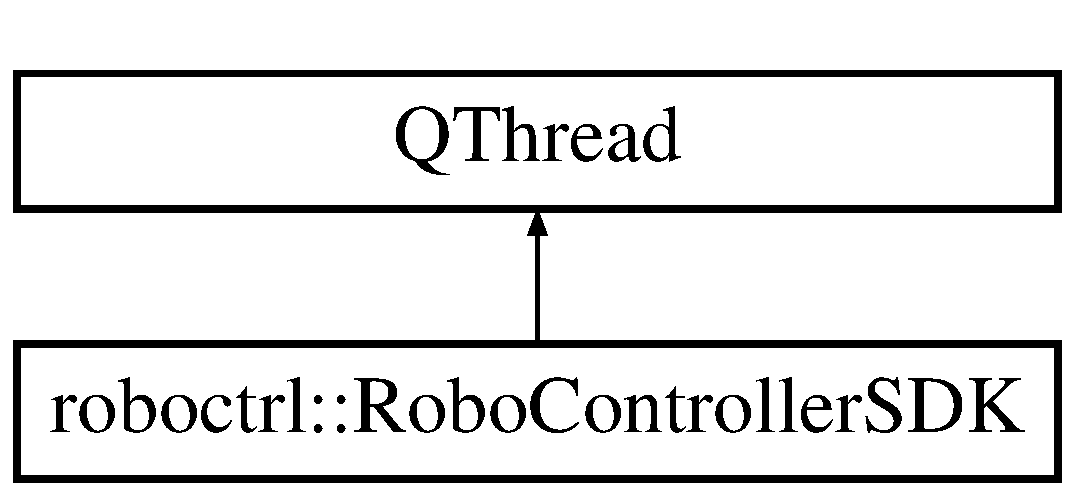
\includegraphics[height=2.000000cm]{classroboctrl_1_1_robo_controller_s_d_k}
\end{center}
\end{figure}
\subsection*{Signals}
\begin{DoxyCompactItemize}
\item 
\hypertarget{classroboctrl_1_1_robo_controller_s_d_k_a9e70ce536b41424c51bc257609b2c675}{void \hyperlink{classroboctrl_1_1_robo_controller_s_d_k_a9e70ce536b41424c51bc257609b2c675}{tcp\-Connected} ()}\label{classroboctrl_1_1_robo_controller_s_d_k_a9e70ce536b41424c51bc257609b2c675}

\begin{DoxyCompactList}\small\item\em Signal emitted when T\-C\-P Socket is connected. \end{DoxyCompactList}\item 
\hypertarget{classroboctrl_1_1_robo_controller_s_d_k_a3e8a1430f0ceca09a3de31b20f02bb5d}{void \hyperlink{classroboctrl_1_1_robo_controller_s_d_k_a3e8a1430f0ceca09a3de31b20f02bb5d}{tcp\-Disconnected} ()}\label{classroboctrl_1_1_robo_controller_s_d_k_a3e8a1430f0ceca09a3de31b20f02bb5d}

\begin{DoxyCompactList}\small\item\em Signal emitted when T\-C\-P Socket is disconnected. \end{DoxyCompactList}\item 
\hypertarget{classroboctrl_1_1_robo_controller_s_d_k_a1c0dbdb62596097a64755fd12670f980}{void \hyperlink{classroboctrl_1_1_robo_controller_s_d_k_a1c0dbdb62596097a64755fd12670f980}{udp\-Connected} ()}\label{classroboctrl_1_1_robo_controller_s_d_k_a1c0dbdb62596097a64755fd12670f980}

\begin{DoxyCompactList}\small\item\em Signal emitted when U\-D\-P Socket is connected. \end{DoxyCompactList}\item 
\hypertarget{classroboctrl_1_1_robo_controller_s_d_k_afefc46c540948597ca05deccac69aceb}{void \hyperlink{classroboctrl_1_1_robo_controller_s_d_k_afefc46c540948597ca05deccac69aceb}{udp\-Disconnected} ()}\label{classroboctrl_1_1_robo_controller_s_d_k_afefc46c540948597ca05deccac69aceb}

\begin{DoxyCompactList}\small\item\em Signal emitted when U\-D\-P Socket is disconnected. \end{DoxyCompactList}\item 
\hypertarget{classroboctrl_1_1_robo_controller_s_d_k_ad86055b34f7c153550ad6984eb527b43}{void \hyperlink{classroboctrl_1_1_robo_controller_s_d_k_ad86055b34f7c153550ad6984eb527b43}{new\-Motor\-Pwm\-Value} (quint16 motor\-Idx, quint16 value)}\label{classroboctrl_1_1_robo_controller_s_d_k_ad86055b34f7c153550ad6984eb527b43}

\begin{DoxyCompactList}\small\item\em Signal emitted when a new P\-W\-M value is received. \end{DoxyCompactList}\item 
\hypertarget{classroboctrl_1_1_robo_controller_s_d_k_abd8a8b44c6abfbc8c74e8ef555f3a6a4}{void \hyperlink{classroboctrl_1_1_robo_controller_s_d_k_abd8a8b44c6abfbc8c74e8ef555f3a6a4}{new\-Motor\-Speed\-Value} (quint16 motor\-Idx, double value)}\label{classroboctrl_1_1_robo_controller_s_d_k_abd8a8b44c6abfbc8c74e8ef555f3a6a4}

\begin{DoxyCompactList}\small\item\em Signal emitted when a new S\-P\-E\-E\-D value is received (speed is in m/sec) \end{DoxyCompactList}\item 
\hypertarget{classroboctrl_1_1_robo_controller_s_d_k_a48a91cbaae37dd8f6ca67c90504c10e9}{void \hyperlink{classroboctrl_1_1_robo_controller_s_d_k_a48a91cbaae37dd8f6ca67c90504c10e9}{new\-Motor\-Pwm\-Value} (quint16 motor\-Idx, double value)}\label{classroboctrl_1_1_robo_controller_s_d_k_a48a91cbaae37dd8f6ca67c90504c10e9}

\begin{DoxyCompactList}\small\item\em Signal emitted when a new P\-W\-M value is received. \end{DoxyCompactList}\item 
\hypertarget{classroboctrl_1_1_robo_controller_s_d_k_a79e70831349070cde327df8ad6be33cb}{void \hyperlink{classroboctrl_1_1_robo_controller_s_d_k_a79e70831349070cde327df8ad6be33cb}{new\-Motor\-P\-I\-D\-Gains} (quint16 motor\-Idx, quint16 Kp, quint16 Ki, quint16 Kd)}\label{classroboctrl_1_1_robo_controller_s_d_k_a79e70831349070cde327df8ad6be33cb}

\begin{DoxyCompactList}\small\item\em Signal emitted when new P\-I\-D gains are received. \end{DoxyCompactList}\item 
\hypertarget{classroboctrl_1_1_robo_controller_s_d_k_a3390df210714579ef9515452780f73ac}{void \hyperlink{classroboctrl_1_1_robo_controller_s_d_k_a3390df210714579ef9515452780f73ac}{new\-Robot\-Configuration} (\hyperlink{struct___robot_configuration}{Robot\-Configuration} \&rob\-Conf)}\label{classroboctrl_1_1_robo_controller_s_d_k_a3390df210714579ef9515452780f73ac}

\begin{DoxyCompactList}\small\item\em Signal emitted when a new Robot Configuration is received from robot. \end{DoxyCompactList}\item 
\hypertarget{classroboctrl_1_1_robo_controller_s_d_k_af760a666eb8e891c0e158e28fab1fb3a}{void \hyperlink{classroboctrl_1_1_robo_controller_s_d_k_af760a666eb8e891c0e158e28fab1fb3a}{new\-Board\-Status} (\hyperlink{struct___board_status}{Board\-Status} \&status)}\label{classroboctrl_1_1_robo_controller_s_d_k_af760a666eb8e891c0e158e28fab1fb3a}

\begin{DoxyCompactList}\small\item\em Signal emitted when a new Board Status is ready. \end{DoxyCompactList}\end{DoxyCompactItemize}
\subsection*{Public Member Functions}
\begin{DoxyCompactItemize}
\item 
\hypertarget{classroboctrl_1_1_robo_controller_s_d_k_a635f633e0d4f0fe8e4da355ded900f61}{{\bfseries Robo\-Controller\-S\-D\-K} (int udp\-Listen\-Port=4550, int udp\-Send\-Port=4560, Q\-String tcp\-Addr=Q\-String(\char`\"{}localhost\char`\"{}), int tcp\-Port=4500)}\label{classroboctrl_1_1_robo_controller_s_d_k_a635f633e0d4f0fe8e4da355ded900f61}

\item 
void \hyperlink{classroboctrl_1_1_robo_controller_s_d_k_aa7e543c9ab8421375f84670184f56168}{set\-Comm\-Mode} (Comm\-Mode mode)
\begin{DoxyCompactList}\small\item\em Sets the current mode. \end{DoxyCompactList}\item 
void \hyperlink{classroboctrl_1_1_robo_controller_s_d_k_a8ff3ba7952c40e6249d6d76ed5e2d5ee}{get\-Motor\-Speed} (quint16 motor\-Idx)
\begin{DoxyCompactList}\small\item\em Send a request for motor speed. The reply is received with /ref new\-Motor\-Speed\-Value signal. \end{DoxyCompactList}\item 
void \hyperlink{classroboctrl_1_1_robo_controller_s_d_k_a975191d6bb8f097e49f3f4a523925550}{set\-Motor\-Speed} (quint16 motor\-Idx, double speed)
\begin{DoxyCompactList}\small\item\em Sets the speed of the motor in m/sec. \end{DoxyCompactList}\item 
void \hyperlink{classroboctrl_1_1_robo_controller_s_d_k_a25ae4287aa49003c5430a0f80870308a}{get\-Motor\-P\-W\-M} (quint16 motor\-Idx)
\begin{DoxyCompactList}\small\item\em Send a request for motor pwm. The reply is received with /ref new\-Motor\-Pwm\-Value signal. \end{DoxyCompactList}\item 
void \hyperlink{classroboctrl_1_1_robo_controller_s_d_k_a4a83d1bb367572c1d0d364eb49fb95ab}{set\-Motor\-P\-W\-M} (quint16 motor\-Idx, int pwm)
\begin{DoxyCompactList}\small\item\em Sets the P\-W\-M of the motor in m/sec. \end{DoxyCompactList}\item 
void \hyperlink{classroboctrl_1_1_robo_controller_s_d_k_a32c9f23fcb8d03b79cbf8745f7bd2324}{set\-Motor\-Pid\-Gains} (quint16 motor\-Idx, quint16 Kp, quint16 Ki, quint16 Kd)
\begin{DoxyCompactList}\small\item\em Sets motor P\-I\-D Controllers parameters. \end{DoxyCompactList}\item 
void \hyperlink{classroboctrl_1_1_robo_controller_s_d_k_a64c0e778ab357964bd84a1f54232d914}{get\-Motor\-Pid\-Gains} (quint16 motor\-Idx)
\begin{DoxyCompactList}\small\item\em Send a request for motor P\-I\-D gains. The reply is received with \hyperlink{classroboctrl_1_1_robo_controller_s_d_k_a79e70831349070cde327df8ad6be33cb}{new\-Motor\-P\-I\-D\-Gains} signal. \end{DoxyCompactList}\item 
\hypertarget{classroboctrl_1_1_robo_controller_s_d_k_a851fd906016bf37f8b2b5580df18811d}{void \hyperlink{classroboctrl_1_1_robo_controller_s_d_k_a851fd906016bf37f8b2b5580df18811d}{get\-Board\-Status} ()}\label{classroboctrl_1_1_robo_controller_s_d_k_a851fd906016bf37f8b2b5580df18811d}

\begin{DoxyCompactList}\small\item\em Gets current board status (Board\-Status) The reply is received with \hyperlink{classroboctrl_1_1_robo_controller_s_d_k_af760a666eb8e891c0e158e28fab1fb3a}{new\-Board\-Status}. \end{DoxyCompactList}\item 
void \hyperlink{classroboctrl_1_1_robo_controller_s_d_k_a39fc9bf4e9444601ec184d542d9faf11}{set\-Board\-Status} (\hyperlink{struct___board_status}{Board\-Status} \&status)
\begin{DoxyCompactList}\small\item\em Sets a new Board\-Status. \end{DoxyCompactList}\item 
bool \hyperlink{classroboctrl_1_1_robo_controller_s_d_k_a4c20cb0043bfcdfb703542081e20eb3b}{get\-Robot\-Configuration\-From\-Ini} (Q\-String ini\-File=R\-O\-B\-O\-T\-\_\-\-C\-O\-N\-F\-I\-G\-\_\-\-I\-N\-I\-\_\-\-F\-I\-L\-E)
\begin{DoxyCompactList}\small\item\em Load the Robot Configuration from ini file The Robot configuration is not stored on Robot E\-E\-P\-R\-O\-M unless saving is active. \end{DoxyCompactList}\item 
\hypertarget{classroboctrl_1_1_robo_controller_s_d_k_a04db4ed91c72189732236ccd9c006564}{void \hyperlink{classroboctrl_1_1_robo_controller_s_d_k_a04db4ed91c72189732236ccd9c006564}{get\-Robot\-Configuration\-From\-Eeprom} ()}\label{classroboctrl_1_1_robo_controller_s_d_k_a04db4ed91c72189732236ccd9c006564}

\begin{DoxyCompactList}\small\item\em Load the Robot Configuration from Robot E\-E\-P\-R\-O\-M The Robot configuration is retrieved from Robot. \end{DoxyCompactList}\item 
void \hyperlink{classroboctrl_1_1_robo_controller_s_d_k_ae032c7eaf9f1074a4f301f04fb30209d}{save\-Robot\-Configuration\-To\-Ini} (Q\-String ini\-File=R\-O\-B\-O\-T\-\_\-\-C\-O\-N\-F\-I\-G\-\_\-\-I\-N\-I\-\_\-\-F\-I\-L\-E)
\begin{DoxyCompactList}\small\item\em Save the Robot Configuration to Robot E\-E\-P\-R\-O\-M The Robot configuration is saved on the Robot. \end{DoxyCompactList}\item 
\hypertarget{classroboctrl_1_1_robo_controller_s_d_k_ae267786e376768c29a3f23bb089ba70c}{void \hyperlink{classroboctrl_1_1_robo_controller_s_d_k_ae267786e376768c29a3f23bb089ba70c}{save\-Robot\-Configuration\-To\-Eeprom} ()}\label{classroboctrl_1_1_robo_controller_s_d_k_ae267786e376768c29a3f23bb089ba70c}

\begin{DoxyCompactList}\small\item\em Save the Robot Configuration to Robot E\-E\-P\-R\-O\-M The Robot configuration is saved on the Robot $\ast$. \end{DoxyCompactList}\end{DoxyCompactItemize}
\subsection*{Protected Slots}
\begin{DoxyCompactItemize}
\item 
\hypertarget{classroboctrl_1_1_robo_controller_s_d_k_a0e317d98289b546c8e4fd3a69bd8840a}{void {\bfseries on\-Tcp\-Ready\-Read} ()}\label{classroboctrl_1_1_robo_controller_s_d_k_a0e317d98289b546c8e4fd3a69bd8840a}

\item 
\hypertarget{classroboctrl_1_1_robo_controller_s_d_k_aa06a7496c69c9c286f96f3d82aef9bc3}{void {\bfseries on\-Tcp\-Error} (Q\-Abstract\-Socket\-::\-Socket\-Error err)}\label{classroboctrl_1_1_robo_controller_s_d_k_aa06a7496c69c9c286f96f3d82aef9bc3}

\item 
\hypertarget{classroboctrl_1_1_robo_controller_s_d_k_a541ff65ff5c39e696532fdb42bf3a166}{void {\bfseries on\-Tcp\-Host\-Found} ()}\label{classroboctrl_1_1_robo_controller_s_d_k_a541ff65ff5c39e696532fdb42bf3a166}

\item 
\hypertarget{classroboctrl_1_1_robo_controller_s_d_k_ac40bcdfb9f6c8780fdba2c7af428485c}{void \hyperlink{classroboctrl_1_1_robo_controller_s_d_k_ac40bcdfb9f6c8780fdba2c7af428485c}{on\-Ping\-Timer\-Timeout} ()}\label{classroboctrl_1_1_robo_controller_s_d_k_ac40bcdfb9f6c8780fdba2c7af428485c}

\begin{DoxyCompactList}\small\item\em Ping Timer handler. \end{DoxyCompactList}\end{DoxyCompactItemize}
\subsection*{Protected Member Functions}
\begin{DoxyCompactItemize}
\item 
virtual void \hyperlink{classroboctrl_1_1_robo_controller_s_d_k_a056d606543ec2a9ba9fd6f151776b72a}{run} ()
\begin{DoxyCompactList}\small\item\em Disables the Communication Watchdog Watch\-Dog if active stops motors if communication is lost. \end{DoxyCompactList}\end{DoxyCompactItemize}


\subsection{Member Function Documentation}
\hypertarget{classroboctrl_1_1_robo_controller_s_d_k_a64c0e778ab357964bd84a1f54232d914}{\index{roboctrl\-::\-Robo\-Controller\-S\-D\-K@{roboctrl\-::\-Robo\-Controller\-S\-D\-K}!get\-Motor\-Pid\-Gains@{get\-Motor\-Pid\-Gains}}
\index{get\-Motor\-Pid\-Gains@{get\-Motor\-Pid\-Gains}!roboctrl::RoboControllerSDK@{roboctrl\-::\-Robo\-Controller\-S\-D\-K}}
\subsubsection[{get\-Motor\-Pid\-Gains}]{\setlength{\rightskip}{0pt plus 5cm}void roboctrl\-::\-Robo\-Controller\-S\-D\-K\-::get\-Motor\-Pid\-Gains (
\begin{DoxyParamCaption}
\item[{quint16}]{motor\-Idx}
\end{DoxyParamCaption}
)}}\label{classroboctrl_1_1_robo_controller_s_d_k_a64c0e778ab357964bd84a1f54232d914}


Send a request for motor P\-I\-D gains. The reply is received with \hyperlink{classroboctrl_1_1_robo_controller_s_d_k_a79e70831349070cde327df8ad6be33cb}{new\-Motor\-P\-I\-D\-Gains} signal. 


\begin{DoxyParams}{Parameters}
{\em motor\-Idx} & Index of the motor (0 or 1) \\
\hline
\end{DoxyParams}
\hypertarget{classroboctrl_1_1_robo_controller_s_d_k_a25ae4287aa49003c5430a0f80870308a}{\index{roboctrl\-::\-Robo\-Controller\-S\-D\-K@{roboctrl\-::\-Robo\-Controller\-S\-D\-K}!get\-Motor\-P\-W\-M@{get\-Motor\-P\-W\-M}}
\index{get\-Motor\-P\-W\-M@{get\-Motor\-P\-W\-M}!roboctrl::RoboControllerSDK@{roboctrl\-::\-Robo\-Controller\-S\-D\-K}}
\subsubsection[{get\-Motor\-P\-W\-M}]{\setlength{\rightskip}{0pt plus 5cm}void roboctrl\-::\-Robo\-Controller\-S\-D\-K\-::get\-Motor\-P\-W\-M (
\begin{DoxyParamCaption}
\item[{quint16}]{motor\-Idx}
\end{DoxyParamCaption}
)}}\label{classroboctrl_1_1_robo_controller_s_d_k_a25ae4287aa49003c5430a0f80870308a}


Send a request for motor pwm. The reply is received with /ref new\-Motor\-Pwm\-Value signal. 


\begin{DoxyParams}{Parameters}
{\em motor\-Idx} & Index of the motor (0 or 1) \\
\hline
\end{DoxyParams}
\hypertarget{classroboctrl_1_1_robo_controller_s_d_k_a8ff3ba7952c40e6249d6d76ed5e2d5ee}{\index{roboctrl\-::\-Robo\-Controller\-S\-D\-K@{roboctrl\-::\-Robo\-Controller\-S\-D\-K}!get\-Motor\-Speed@{get\-Motor\-Speed}}
\index{get\-Motor\-Speed@{get\-Motor\-Speed}!roboctrl::RoboControllerSDK@{roboctrl\-::\-Robo\-Controller\-S\-D\-K}}
\subsubsection[{get\-Motor\-Speed}]{\setlength{\rightskip}{0pt plus 5cm}void roboctrl\-::\-Robo\-Controller\-S\-D\-K\-::get\-Motor\-Speed (
\begin{DoxyParamCaption}
\item[{quint16}]{motor\-Idx}
\end{DoxyParamCaption}
)}}\label{classroboctrl_1_1_robo_controller_s_d_k_a8ff3ba7952c40e6249d6d76ed5e2d5ee}


Send a request for motor speed. The reply is received with /ref new\-Motor\-Speed\-Value signal. 


\begin{DoxyParams}{Parameters}
{\em motor\-Idx} & Index of the motor (0 or 1) \\
\hline
\end{DoxyParams}
\hypertarget{classroboctrl_1_1_robo_controller_s_d_k_a4c20cb0043bfcdfb703542081e20eb3b}{\index{roboctrl\-::\-Robo\-Controller\-S\-D\-K@{roboctrl\-::\-Robo\-Controller\-S\-D\-K}!get\-Robot\-Configuration\-From\-Ini@{get\-Robot\-Configuration\-From\-Ini}}
\index{get\-Robot\-Configuration\-From\-Ini@{get\-Robot\-Configuration\-From\-Ini}!roboctrl::RoboControllerSDK@{roboctrl\-::\-Robo\-Controller\-S\-D\-K}}
\subsubsection[{get\-Robot\-Configuration\-From\-Ini}]{\setlength{\rightskip}{0pt plus 5cm}bool roboctrl\-::\-Robo\-Controller\-S\-D\-K\-::get\-Robot\-Configuration\-From\-Ini (
\begin{DoxyParamCaption}
\item[{Q\-String}]{ini\-File = {\ttfamily ROBOT\-\_\-CONFIG\-\_\-INI\-\_\-FILE}}
\end{DoxyParamCaption}
)}}\label{classroboctrl_1_1_robo_controller_s_d_k_a4c20cb0043bfcdfb703542081e20eb3b}


Load the Robot Configuration from ini file The Robot configuration is not stored on Robot E\-E\-P\-R\-O\-M unless saving is active. 


\begin{DoxyParams}{Parameters}
{\em ini\-File} & The path of the ini file\\
\hline
\end{DoxyParams}
\begin{DoxyReturn}{Returns}
true if everything is ok 
\end{DoxyReturn}
\hypertarget{classroboctrl_1_1_robo_controller_s_d_k_a056d606543ec2a9ba9fd6f151776b72a}{\index{roboctrl\-::\-Robo\-Controller\-S\-D\-K@{roboctrl\-::\-Robo\-Controller\-S\-D\-K}!run@{run}}
\index{run@{run}!roboctrl::RoboControllerSDK@{roboctrl\-::\-Robo\-Controller\-S\-D\-K}}
\subsubsection[{run}]{\setlength{\rightskip}{0pt plus 5cm}void roboctrl\-::\-Robo\-Controller\-S\-D\-K\-::run (
\begin{DoxyParamCaption}
{}
\end{DoxyParamCaption}
)\hspace{0.3cm}{\ttfamily [protected]}, {\ttfamily [virtual]}}}\label{classroboctrl_1_1_robo_controller_s_d_k_a056d606543ec2a9ba9fd6f151776b72a}


Disables the Communication Watchdog Watch\-Dog if active stops motors if communication is lost. 

Enables the Communication Watchdog Watch\-Dog if active stops motors if communication is lost\-Thread function \hypertarget{classroboctrl_1_1_robo_controller_s_d_k_ae032c7eaf9f1074a4f301f04fb30209d}{\index{roboctrl\-::\-Robo\-Controller\-S\-D\-K@{roboctrl\-::\-Robo\-Controller\-S\-D\-K}!save\-Robot\-Configuration\-To\-Ini@{save\-Robot\-Configuration\-To\-Ini}}
\index{save\-Robot\-Configuration\-To\-Ini@{save\-Robot\-Configuration\-To\-Ini}!roboctrl::RoboControllerSDK@{roboctrl\-::\-Robo\-Controller\-S\-D\-K}}
\subsubsection[{save\-Robot\-Configuration\-To\-Ini}]{\setlength{\rightskip}{0pt plus 5cm}void roboctrl\-::\-Robo\-Controller\-S\-D\-K\-::save\-Robot\-Configuration\-To\-Ini (
\begin{DoxyParamCaption}
\item[{Q\-String}]{ini\-File = {\ttfamily ROBOT\-\_\-CONFIG\-\_\-INI\-\_\-FILE}}
\end{DoxyParamCaption}
)}}\label{classroboctrl_1_1_robo_controller_s_d_k_ae032c7eaf9f1074a4f301f04fb30209d}


Save the Robot Configuration to Robot E\-E\-P\-R\-O\-M The Robot configuration is saved on the Robot. 


\begin{DoxyParams}{Parameters}
{\em ini\-File} & The path of the ini file \\
\hline
\end{DoxyParams}
\hypertarget{classroboctrl_1_1_robo_controller_s_d_k_a39fc9bf4e9444601ec184d542d9faf11}{\index{roboctrl\-::\-Robo\-Controller\-S\-D\-K@{roboctrl\-::\-Robo\-Controller\-S\-D\-K}!set\-Board\-Status@{set\-Board\-Status}}
\index{set\-Board\-Status@{set\-Board\-Status}!roboctrl::RoboControllerSDK@{roboctrl\-::\-Robo\-Controller\-S\-D\-K}}
\subsubsection[{set\-Board\-Status}]{\setlength{\rightskip}{0pt plus 5cm}void roboctrl\-::\-Robo\-Controller\-S\-D\-K\-::set\-Board\-Status (
\begin{DoxyParamCaption}
\item[{{\bf Board\-Status} \&}]{status}
\end{DoxyParamCaption}
)}}\label{classroboctrl_1_1_robo_controller_s_d_k_a39fc9bf4e9444601ec184d542d9faf11}


Sets a new Board\-Status. 


\begin{DoxyParams}{Parameters}
{\em status} & The new status to be set \\
\hline
\end{DoxyParams}
\hypertarget{classroboctrl_1_1_robo_controller_s_d_k_aa7e543c9ab8421375f84670184f56168}{\index{roboctrl\-::\-Robo\-Controller\-S\-D\-K@{roboctrl\-::\-Robo\-Controller\-S\-D\-K}!set\-Comm\-Mode@{set\-Comm\-Mode}}
\index{set\-Comm\-Mode@{set\-Comm\-Mode}!roboctrl::RoboControllerSDK@{roboctrl\-::\-Robo\-Controller\-S\-D\-K}}
\subsubsection[{set\-Comm\-Mode}]{\setlength{\rightskip}{0pt plus 5cm}void roboctrl\-::\-Robo\-Controller\-S\-D\-K\-::set\-Comm\-Mode (
\begin{DoxyParamCaption}
\item[{Comm\-Mode}]{mode}
\end{DoxyParamCaption}
)}}\label{classroboctrl_1_1_robo_controller_s_d_k_aa7e543c9ab8421375f84670184f56168}


Sets the current mode. 

Disables the Communication Watchdog.


\begin{DoxyParams}{Parameters}
{\em mode} & The mode to be set. See Comm\-Mode\\
\hline
\end{DoxyParams}

\begin{DoxyExceptions}{Exceptions}
{\em \hyperlink{classroboctrl_1_1_rc_exception}{Rc\-Exception}} & Enables the Communication Watchdog \\
\hline
\end{DoxyExceptions}
\hypertarget{classroboctrl_1_1_robo_controller_s_d_k_a32c9f23fcb8d03b79cbf8745f7bd2324}{\index{roboctrl\-::\-Robo\-Controller\-S\-D\-K@{roboctrl\-::\-Robo\-Controller\-S\-D\-K}!set\-Motor\-Pid\-Gains@{set\-Motor\-Pid\-Gains}}
\index{set\-Motor\-Pid\-Gains@{set\-Motor\-Pid\-Gains}!roboctrl::RoboControllerSDK@{roboctrl\-::\-Robo\-Controller\-S\-D\-K}}
\subsubsection[{set\-Motor\-Pid\-Gains}]{\setlength{\rightskip}{0pt plus 5cm}void roboctrl\-::\-Robo\-Controller\-S\-D\-K\-::set\-Motor\-Pid\-Gains (
\begin{DoxyParamCaption}
\item[{quint16}]{motor\-Idx, }
\item[{quint16}]{Kp, }
\item[{quint16}]{Ki, }
\item[{quint16}]{Kd}
\end{DoxyParamCaption}
)}}\label{classroboctrl_1_1_robo_controller_s_d_k_a32c9f23fcb8d03b79cbf8745f7bd2324}


Sets motor P\-I\-D Controllers parameters. 


\begin{DoxyParams}{Parameters}
{\em motor\-Idx} & Index of the motor (0 or 1) \\
\hline
{\em Kp} & Proportional Action gain \\
\hline
{\em Ki} & Integral Action gain \\
\hline
{\em Kd} & Derivative Action gain \\
\hline
\end{DoxyParams}
\hypertarget{classroboctrl_1_1_robo_controller_s_d_k_a4a83d1bb367572c1d0d364eb49fb95ab}{\index{roboctrl\-::\-Robo\-Controller\-S\-D\-K@{roboctrl\-::\-Robo\-Controller\-S\-D\-K}!set\-Motor\-P\-W\-M@{set\-Motor\-P\-W\-M}}
\index{set\-Motor\-P\-W\-M@{set\-Motor\-P\-W\-M}!roboctrl::RoboControllerSDK@{roboctrl\-::\-Robo\-Controller\-S\-D\-K}}
\subsubsection[{set\-Motor\-P\-W\-M}]{\setlength{\rightskip}{0pt plus 5cm}void roboctrl\-::\-Robo\-Controller\-S\-D\-K\-::set\-Motor\-P\-W\-M (
\begin{DoxyParamCaption}
\item[{quint16}]{motor\-Idx, }
\item[{int}]{pwm}
\end{DoxyParamCaption}
)}}\label{classroboctrl_1_1_robo_controller_s_d_k_a4a83d1bb367572c1d0d364eb49fb95ab}


Sets the P\-W\-M of the motor in m/sec. 


\begin{DoxyParams}{Parameters}
{\em motor\-Idx} & Index of the motor (0 or 1) \\
\hline
{\em pwm} & P\-W\-M range\-: \mbox{[}-\/2048/2047\mbox{]}\\
\hline
\end{DoxyParams}
\begin{DoxyNote}{Note}
This function works only when m\-Motor\-Ctrl\-Mode is equal to mc\-Pid, else it does nothing 
\end{DoxyNote}
\hypertarget{classroboctrl_1_1_robo_controller_s_d_k_a975191d6bb8f097e49f3f4a523925550}{\index{roboctrl\-::\-Robo\-Controller\-S\-D\-K@{roboctrl\-::\-Robo\-Controller\-S\-D\-K}!set\-Motor\-Speed@{set\-Motor\-Speed}}
\index{set\-Motor\-Speed@{set\-Motor\-Speed}!roboctrl::RoboControllerSDK@{roboctrl\-::\-Robo\-Controller\-S\-D\-K}}
\subsubsection[{set\-Motor\-Speed}]{\setlength{\rightskip}{0pt plus 5cm}void roboctrl\-::\-Robo\-Controller\-S\-D\-K\-::set\-Motor\-Speed (
\begin{DoxyParamCaption}
\item[{quint16}]{motor\-Idx, }
\item[{double}]{speed}
\end{DoxyParamCaption}
)}}\label{classroboctrl_1_1_robo_controller_s_d_k_a975191d6bb8f097e49f3f4a523925550}


Sets the speed of the motor in m/sec. 


\begin{DoxyParams}{Parameters}
{\em motor\-Idx} & Index of the motor (0 or 1) \\
\hline
{\em speed} & The speed in m/sec -\/ Speed range\-: \mbox{[}-\/32.\-768/+32.767\mbox{]} m/sec\\
\hline
\end{DoxyParams}
\begin{DoxyNote}{Note}
This function works only when m\-Motor\-Ctrl\-Mode is equal to mc\-Pid, else it does nothing 
\end{DoxyNote}


The documentation for this class was generated from the following files\-:\begin{DoxyCompactItemize}
\item 
robocontrollersdk.\-h\item 
robocontrollersdk.\-cpp\end{DoxyCompactItemize}

%--- End generated contents ---

% Index
\newpage
\phantomsection
\addcontentsline{toc}{part}{Index}
\printindex

\end{document}
